%!TEX root = ../main.tex
%%%%%%%%%%%%%%%%%%%%%%%%%%%%%%%%%%
% Links:
% http://www.zrzahid.com/the-%E2%80%A9maximum%E2%80%A9-gap%E2%80%A9-problem-%E2%80%A9pigeonhole-%E2%80%A9principle%E2%80%A9/
% https://leetcode.com/problems/maximum-gap/discuss/50667/Solutions-in-C%2B%2B-with-explanation-read-it-and-then-you-get-it
% https://leetcode.com/problems/maximum-gap/discuss/50694/12ms-C%2B%2B-Suggested-Solution
% Difficulty: Companies: 
%%%%%%%%%%%%%%%%%%%%%%%%%%%%%%%%%%


%\begin{figure} \centering 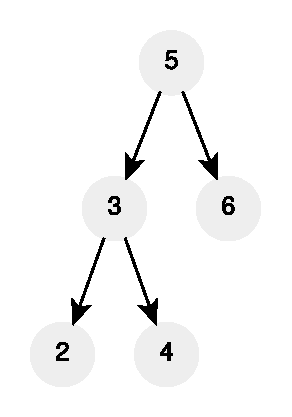
\includegraphics[width=\textwidth]{sources/max_gap/images/example1}
%   \caption[Sample short cpation]{Sample Caption}. \label{fig:max_gap:example1} \end{figure}

\chapter{Find the largest gap}
\label{ch:max_gap}
\section*{Introduction}
The problem discussed in the chapter is another one about sorting. Its statement is quite simple and
the only input given is an unsorted array from which we are asked to calculate a value would be
trivial to find if the input was sorted. Therefore, the real challenge of this problem is to come-up
with a solution that does not require explicit sorting.

Particular attention should be paid to the examples as well as to the problem statement because it
is quite easy to misinterpret the real requirements of the function you asked to write if you dive
right away into coding. The problem asks you to return the largest distance between any element in
the input array provided they appear one next to the other when $I$ is sorted. You might
misinterpret the problem by thinking that you need to return the largest distance between any two
elements of the original input array. This interpretation is wrong, and your intuition should make
you aware of it right away considering that the solution to this problem involves only finding the
minimum and the maximum values of the input array. You can expect any coding interview question to
be harder than that. An imagination effort (or some pen and paper work) is thus necessary to
understand each of the examples provided.

\section{Problem statement}
\begin{exercise}
\label{example:max_gap:exercice1}
Write a function that given a unsorted array of non-negative integers 
$I$ of length $n$ returns the largest gap between two
elements that would appear one next to the other  
if $I$ was sorted. A gap between $x$ and $y$ is defined as the absolute value of the difference
between $x$ and $y$: $|x-y|$.

	%example1
	\begin{example}
		\label{example:max_gap:example1}
		\hfill \\
		Given $I = \{5,3,1,8,9,2,4\}$ the function returns $3$. Sorting $I$ changes it into:
		$sort(I)= \{1,2,3,4,5,8,9\}$, and the largest gap between any two consecutive elements is
		$3$. In this case between $5$ and $8$.		
	\end{example}

	%example2
	\begin{example}
		\label{example:max_gap:example2}
		\hfill \\
		Given $I = \{7, 1, 8, 9,15\}$ the function returns $6$. $sort(I)= \{1,7,8,9,15\}$, and the
		largest gap between any two of its consecutive elements is $6$ e.g. between $1$ and $7$ or
		between $15$ and $9$.	
	\end{example}
	
\end{exercise}

\section{Clarification Questions}

\begin{QandA}
	\item Is the input $I$ modifiable?
	\begin{answered}
		\textit{Yes you can modify $I$.}
	\end{answered}

	\item Is any guarantee or constraint on the value of each element of $I$?
	\begin{answered}
		\textit{You can assume each element of $I$ to fit in a 4 bytes unsigned integer.}
	\end{answered}
	
\end{QandA}

%\section{Discussion} \label{max_gap:sec:discussion}


\section{Trivial Solution}
\label{max_gap:sec:trivial}
As already mentioned in the introduction this problem has an extremely simple solution when we can
afford to get our hands on a sorted version of the input array. In this specific version of the
problem $I$ is not read-only and we are allowed to modify it,therefore, we can sort it directly. If
that is not possible all you have to do is to create a copy of $I$ and sort that instead. 

Given a sorted collection, the largest gap between any two numbers can be find in linear time by
just scanning each pair $p=(I_k, I_{k+1)}$ of subsequent elements and for each of them calculate
their distance $d_k=I_{k-1}-I_k$. Among all calculated distances we just return the largest. Listing
\ref{list:max_gap:bruteforce} shows an implementation of this idea. Notice that:
\begin{itemize}
	\item we do not need to use the absolute value operation as we are operating on a sorted
	collection and therefore, we are guaranteed that $I_{k+1}$ is larger or equal than $I_k$.
	\item the \inline{for} loop stops when $i=|I|-1$ in order to avoid accessing an invalid element
	while executing \inline{I_copy[i+1]}. When $i=|I|-1$ this would lead to accessing the element at index
	$|I|$, which does not exists. In C++ this would cause undefined behaviour, and the most likely
	outcome would be a segmentation fault error.
\end{itemize}
\lstinputlisting[language=c++, caption={Trivial solution to the max gap problem using sorting and linear space.},label=list:max_gap:bruteforce]{sources/max_gap/max_gap_solution1.cpp}



\section{Radix Sort}
\label{max_gap:sec:radix_sort}
The idea we developed in Section \ref{max_gap:sec:trivial} can be improved 
if instead of using a normal comparison-based sorting algorithm  we use 
radix-sort\cite{cit::wiki::radix_sort }instead. 
Radix sort will perform better than a standard $O(nlogn)$ algorithm when there is an upper bound for the values of the 
input array. If we assume that such bound is the largest value a standard 4 bytes \inline{int} can hold then radix sort will 
have a complexity of $O(n)$.

Radix sort works by sorting the input array $d$ times, where $d = \floor{log_{10}k+1}$ and $k$ is the largest number in $I$.
$d$ is just the number of digits of the largest number in the list. For a standard \inline{int} $d=\floor{log_{10}(2147483647) + 1}=10$.
The sorting is obtained by repeatedly sorting the input list from the least to the most significant digit where each of the intermediate 
sorting steps is performed using counting-sort.
For instance given $I = \{329,457,657,839,436,720,355\}$ the first pass of radix sort will sort $I$ based on the value of the least significant digits.
After this first pass we have $I=\{720,355,436,457,657,329,839\}$. Notice how the first digits are sorted. At this point the algorithm proceed by sorting 
$I$ further but this time according to their second digit. The resulting list becomes $I=\{720,329,436,839,355,457,657\}$.
Finally the third pass will sort all the elements according the the most significant digit, resulting in a well
sorted list: $I=\{329,355,436,457,657,720,839\}$. 
Notice that this approach needs to be tweaked in case you want to apply radix sort to negative numbers\footnote{You can treat the sign as a special kind of digit. 
You sort the pile on the units, then the tens, etc. and finally on the sign. 
This does produce a reversed order for the negatives, 
you then simply reverse the contents of that bucket.}.

Listing \ref{list:max_gap:radixsort} shows an implementation of radix-sort and its application to the solution of this chapter's problem.
\lstinputlisting[language=c++, caption={Linear time solution to the max gap problem using radix-sort.},label=list:max_gap:radixsort]{sources/max_gap/max_gap_solution2.cpp}
Notice how the main driver function \inline{max_gap_radix_sort} is basically the same as \inline{max_gap_bruteforce} from Listing \ref{list:max_gap:bruteforce} except for the sorting procedure used.

\section{Buckets and the pigeonhole principle}
\label{max_gap:sec:buckets}
All the solutions we have presented so far rely on sorting. In this section we are going to discuss an approach
that rely on  the pigeonhole principle\footnote{\url{https://en.wikipedia.org/wiki/Pigeonhole_principle}} and bucketing.
The general idea is that we could split the entire array into several buckets and then find the largest gap by only comparing
one element of a given bucket to one element of the subsequent bucket. 

You can think of $I$ as an array of buckets each containing a single element. $|I|$ is made of $b$ buckets and the total amount of element in $I$ is $n=b$.
Imagine for a moment that you would reduce the number of buckets from $b$ to some integer $k < b$.
For the pigeonhole principle then, one or more of the buckets in $I$ have to contain  strictly more than one element.

Let's now focus for a moment of the gaps of an ideal collection where each of the elements has a given distance $t$ from its successor in the list. 
If such a collection ic composed of  $n$ elements, then there is a total of $n-1$ gaps, each of size $t$.
$t$ can be easily calculate if the maximum and minimum values are known: in-fact $t=\frac{max-min}{n-1}$. 
If $I$ was like this ideal collection then the problem would be easily solved by using the formula above. 
$I$ is different to this ideal collection because elements do not have uniform gaps between each other. 
In this situation then we can argue that the maximum gap between any pair of subsequent 
elements of $I$ is always larger than $t$.
We can show this by trying reduce the gap between two subsequent elements $I_{i}$ and $I_{i+1}$, of an ideal collection with uniform gaps.
We can do that by moving $I_{i+1}$ closer to $I_{i}$. When this happens the gap $(I_{i+1}-I_{i})$ becomes smaller than $t$. But what happens to the gap between $I_{i+1}$ and $I_{i+2}$?
It actually becomes larger than $t$. In our effort to make the largest gap among two subsequent elements smaller, we obtained the opposite result: we made it larger.
This shows that the maximum attainable gap can in a  collection with uniform gaps can only increase. 

We are going to apply the two ideas above to solve this problem in the following way. We will distribute all the element of $I$
into $n-1$ buckets. The first bucket would contains all the elements of $I$ which have in the following range: $[min, min + t)$.
Similarly the second buckets would contain all the elements in the following range: $[min + t, min + 2t)$. 
In general the $i^{th}$ bucket  would contain all the elements of $I$ in the following range: $[min + (i-1)t, min +it)$ (where $ 1 \leq i$).
You can refer to Figure \ref{fig:max_gap:bucketing_example2} for an example of how such a division into buckets would work for the input array in Example \ref{example:max_gap:example2}.
This allows us to skip comparing all the element within a bucket because we know for sure they will have a distance that is lower of equal than $t$ and we can therefore only concentrate on comparing elements 
of subsequent buckets.
In particular we should compare the maximum value of the $i^{th}$ bucket with the minimum value of the $(i+1)^{th}$ bucket. Why? Because they would appear one next to the other if $I$ was sorted.
Because the number of buckets is always lower of equal than the number of elements in the collection, this approach has a linear complexity as it does require to compare at most twice the number of input elements in $I$.


\begin{figure}
	 \centering
	 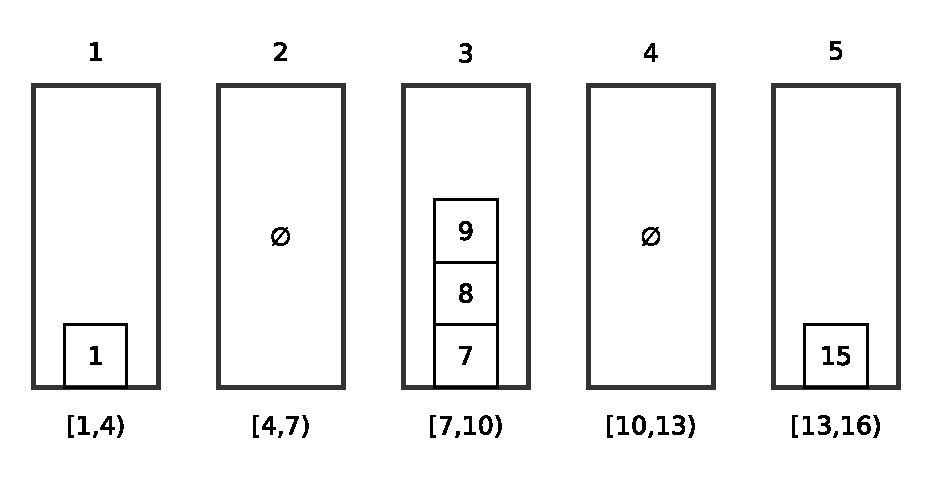
\includegraphics[width=\textwidth]{sources/max_gap/images/bucketing_example1}
     \caption{Division of the elements of the Example \ref{example:max_gap:example2} into buckets.}.
	\label{fig:max_gap:bucketing_example2}
\end{figure}

